\documentclass[journal,twoside,web,onecolumn]{ieeecolor}
\usepackage{generic}
\usepackage{amsmath,amssymb,booktabs,siunitx}
\usepackage[hidelinks]{hyperref}
\usepackage{placeins}
\usepackage{graphicx}
\usepackage{tikz}
\usetikzlibrary{positioning,arrows.meta}
\usetikzlibrary{calc}
\renewcommand{\thetable}{S\arabic{table}}
\renewcommand{\thefigure}{S\arabic{figure}}
\renewcommand{\thesection}{S\arabic{section}}
\makeatletter\let\inputtab\@@input\makeatother

\begin{document}
\sloppy
\title{Supplementary Material for ``Topological Segmentation Error and Boundary-Condition Tuning in Computed Coronary
FFR: A Controlled In Silico Study''}
\author{Fadillah Yamin, Mohd Azan Mohammed Sapardi, Ming Kwang Tan, Xin Wang, and \mbox{Mohd-Zulhilmi Ismadi}\endgraf\vspace{-\baselineskip}}
\markboth{IEEE Journal of Biomedical and Health Informatics}{Yamin \MakeLowercase{\textit{et al.}}: Supplementary Material, Segmentation Error and BC Tuning in Coronary FFR}
\maketitle

\section{Analysis Pipeline}
Fig.~\ref{fig:pipeline} shows the analysis pipeline. The reduced-order arm
runs end to end without manual intervention: every instance, error type, protocol and bed is solved in one automated run
from the cohort list, and every table and figure is generated from its output. The 3D case study is a separate
branch. A case package (centerline, outlet boundary conditions and probe positions) is exported to the CFD machine,
which returns the solved FFR and the as-meshed radius; the radius is used to rebuild the reduced-order counterpart.

Cohort selection (step 3) shuffles the 6\,944 instances with a fixed seed (20260918) and fills the six bands of
leaky-bed baseline FFR scarcest first, rotating the host vessel type and taking at most two instances per tree and
one per host vessel and band. Each host vessel keeps only the lesion positions and lengths that meet the eligibility
criteria, so it contributes fewer than 32 instances when a criterion fails at one position. The reduced-order solve (step 7)
starts from Poiseuille flow, averages successive flow iterates with a relaxation factor of 0.5, and stops when the
largest flow change falls below $10^{-8}$ of the largest flow or after 200 iterations; a solve that reaches the
cap is recorded as not converged, and none did.
\begin{figure}[!h]
\centering
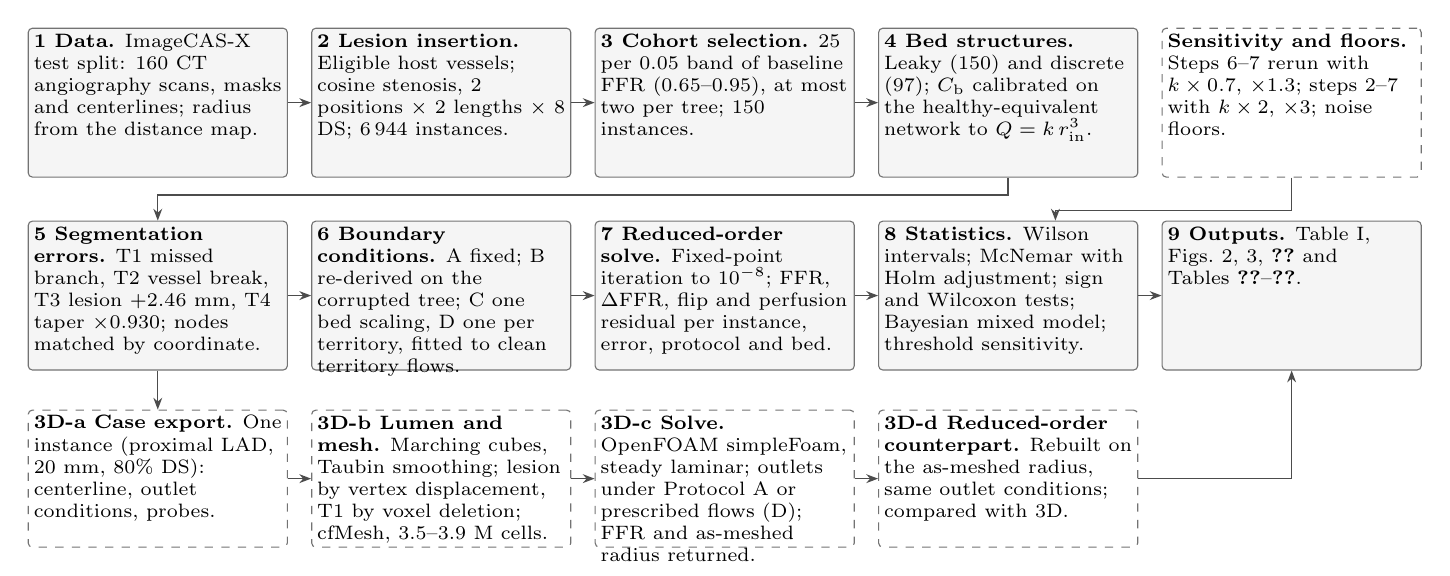
\begin{tikzpicture}[font=\scriptsize, node distance=6mm and 2.6mm,
  box/.style={draw=black!55, fill=black!4, rounded corners=1.5pt, inner sep=2pt, anchor=north west},
  cfd/.style={box, fill=white, dashed},
  arr/.style={-{Stealth[length=1.5mm]}, draw=black!70, line width=0.5pt}]
\def\px{3.6}
\node[box] (data) at (0,0) {\parbox[t][1.75cm][t]{3.15cm}{\raggedright \textbf{1 Data.} \mbox{ImageCAS-X} test split: 160 CT angiography scans, masks and
  centerlines; radius from the distance map.}};
\node[box] (sweep) at (\px,0) {\parbox[t][1.75cm][t]{3.15cm}{\raggedright \textbf{2 Lesion insertion.} Eligible host vessels; cosine stenosis, 2 positions
  $\times$ 2 lengths $\times$ 8 DS; 6\,944 instances.}};
\node[box] (select) at (2*\px,0) {\parbox[t][1.75cm][t]{3.15cm}{\raggedright \textbf{3 Cohort selection.} 25 per 0.05 band of baseline FFR (0.65--0.95), at
  most two per tree; 150 instances.}};
\node[box] (bed) at (3*\px,0) {\parbox[t][1.75cm][t]{3.15cm}{\raggedright \textbf{4 Bed structures.} Leaky (150) and discrete (97); $C_\mathrm{b}$ calibrated on the
  healthy-equivalent network to $Q = k\,r_\mathrm{in}^3$.}};
\node[box, dashed, fill=white] (sens) at (4*\px,0) {\parbox[t][1.75cm][t]{3.15cm}{\raggedright \textbf{Sensitivity and floors.} Steps 6--7 rerun with
  $k \times 0.7$, $\times 1.3$; steps 2--7 with $k \times 2$, $\times 3$; noise floors.}};
\node[box] (err) at (0,-2.45) {\parbox[t][1.75cm][t]{3.15cm}{\raggedright \textbf{5 Segmentation errors.} T1 missed branch, T2 vessel break, T3 lesion
  $+2.46$~mm, T4 taper $\times 0.930$; nodes matched by coordinate.}};
\node[box] (prot) at (\px,-2.45) {\parbox[t][1.75cm][t]{3.15cm}{\raggedright \textbf{6 Boundary conditions.} A fixed; B re-derived on the corrupted tree;
  C one bed scaling, D one per territory, fitted to clean territory flows.}};
\node[box] (solve) at (2*\px,-2.45) {\parbox[t][1.75cm][t]{3.15cm}{\raggedright \textbf{7 Reduced-order solve.} Fixed-point iteration to $10^{-8}$;
  FFR, $\Delta$FFR, flip and perfusion residual per instance, error, protocol and bed.}};
\node[box] (stats) at (3*\px,-2.45) {\parbox[t][1.75cm][t]{3.15cm}{\raggedright \textbf{8 Statistics.} Wilson intervals; McNemar with Holm adjustment; sign
  and Wilcoxon tests; Bayesian mixed model; threshold sensitivity.}};
\node[box] (out) at (4*\px,-2.45) {\parbox[t][1.75cm][t]{3.15cm}{\raggedright \textbf{9 Outputs.} Table I, Figs.~2, 3, \ref{fig:branch} and Tables~\mbox{\ref{tab:excl}--\ref{tab:floor}}.}};
\node[cfd] (exp) at (0,-4.85) {\parbox[t][1.6cm][t]{3.15cm}{\raggedright \textbf{3D-a Case export.} One instance (proximal LAD, 20~mm, 80\% DS): centerline,
  outlet conditions, probes.}};
\node[cfd] (mesh) at (\px,-4.85) {\parbox[t][1.6cm][t]{3.15cm}{\raggedright \textbf{3D-b Lumen and mesh.} Marching cubes, Taubin smoothing; lesion by vertex
  displacement, T1 by voxel deletion; cfMesh, 3.5--3.9~M cells.}};
\node[cfd] (foam) at (2*\px,-4.85) {\parbox[t][1.6cm][t]{3.15cm}{\raggedright \textbf{3D-c Solve.} OpenFOAM simpleFoam, steady laminar; outlets under
  Protocol A or prescribed flows (D); FFR and as-meshed radius returned.}};
\node[cfd] (twin) at (3*\px,-4.85) {\parbox[t][1.6cm][t]{3.15cm}{\raggedright \textbf{3D-d Reduced-order counterpart.} Rebuilt on the as-meshed radius, same outlet
  conditions; compared with 3D.}};
\foreach \u/\v in {data/sweep, sweep/select, select/bed, err/prot, prot/solve, solve/stats, stats/out,
  exp/mesh, mesh/foam, foam/twin} \draw[arr] (\u) -- (\v);
\draw[arr] (bed.south) -- ++(0,-0.22) -| (err.north);
\draw[arr] (sens.south) -- ++(0,-0.42) -| ([xshift=6mm]stats.north);
\draw[arr] (err.south) -- (exp.north);
\draw[arr] (twin.east) -| (out.south);
\end{tikzpicture}
\caption{Analysis pipeline. Shaded boxes: reduced-order arm, run for every
instance. Dashed boxes: sensitivity and noise-floor analyses (top right) and the 3D case study (bottom row), whose
steps 3D-b and 3D-c ran on the CFD machine.}\label{fig:pipeline}
\end{figure}

Fig.~\ref{fig:stenosis} shows the inserted stenosis on one host vessel. The narrowing follows (1) of the main text: it
is set by the taper-fit radius $r_\mathrm{fit}$, not by the local image radius $r$, and the lumen is never
widened.
\begin{figure}[!ht]
\centering
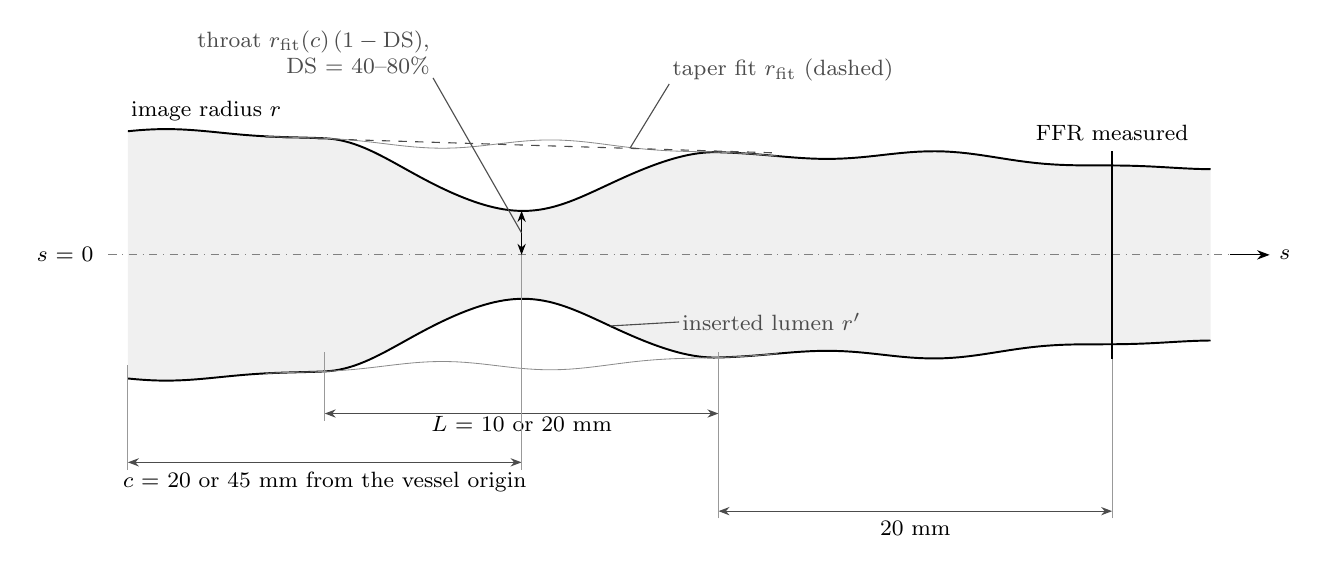
\begin{tikzpicture}[x=1.25cm, y=1.55cm, font=\footnotesize,
  dim/.style={{Stealth[length=1.4mm]}-{Stealth[length=1.4mm]}, line width=0.4pt, draw=black!70}]
\def\c{4}\def\L{4}\def\DS{0.6}
\pgfmathdeclarefunction{rfit}{1}{\pgfmathparse{1.0-0.025*#1}}
\pgfmathdeclarefunction{rimg}{1}{\pgfmathparse{rfit(#1)+0.035*sin(97*#1)+0.02*sin(181*#1+40)}}
\pgfmathdeclarefunction{rles}{1}{\pgfmathparse{min(rimg(#1),(1-0.5*(1+cos(360*(#1-\c)/\L)))*rimg(#1)
  +0.5*(1+cos(360*(#1-\c)/\L))*rfit(#1)*(1-\DS))}}
\fill[black!6] plot[domain=0:\c-\L/2, samples=40] (\x,{rimg(\x)}) -- plot[domain=\c-\L/2:\c+\L/2, samples=80] (\x,{rles(\x)})
  -- plot[domain=\c+\L/2:11, samples=60] (\x,{rimg(\x)}) -- plot[domain=11:\c+\L/2, samples=60] (\x,{-rimg(\x)})
  -- plot[domain=\c+\L/2:\c-\L/2, samples=80] (\x,{-rles(\x)}) -- plot[domain=\c-\L/2:0, samples=40] (\x,{-rimg(\x)}) -- cycle;
\foreach \sg in {1,-1} {
  \draw[line width=0.7pt] plot[domain=0:\c-\L/2, samples=40] (\x,{\sg*rimg(\x)});
  \draw[line width=0.7pt] plot[domain=\c-\L/2:\c+\L/2, samples=80] (\x,{\sg*rles(\x)});
  \draw[line width=0.7pt] plot[domain=\c+\L/2:11, samples=60] (\x,{\sg*rimg(\x)});
  \draw[black!45, line width=0.3pt] plot[domain=\c-\L/2-0.6:\c+\L/2+0.6, samples=60] (\x,{\sg*rimg(\x)});
}
\draw[dashed, black!70] plot[domain=\c-\L/2-0.6:\c+\L/2+0.6, samples=2] (\x,{rfit(\x)});
\draw[dash dot, black!50] (-0.2,0) -- (11.2,0);
\draw[dim] (\c-\L/2,-1.3) -- node[below, fill=white, inner sep=1pt] {$L$ = 10 or 20 mm} (\c+\L/2,-1.3);
\foreach \xx in {\c-\L/2,\c+\L/2} \draw[black!40] (\xx,-1.36) -- (\xx,-0.8);
\draw[dim] (0,-1.7) -- node[below] {$c$ = 20 or 45 mm from the vessel origin} (\c,-1.7);
\draw[black!40] (0,-1.76) -- (0,-0.9); \draw[black!40] (\c,-1.76) -- (\c,0);
\draw[{Stealth[length=1.4mm]}-{Stealth[length=1.4mm]}, line width=0.4pt] (\c,0) -- (\c,{rles(\c)});
\draw[black!70] (\c,{0.5*rles(\c)}) -- (\c-0.9,1.45) node[anchor=south east, inner sep=1pt, align=right] {throat $r_\mathrm{fit}(c)\,(1-\mathrm{DS})$,\\ DS = 40--80\%};
\node[anchor=south west, inner sep=1pt] at (0,{rimg(0)+0.06}) {image radius $r$};
\draw[black!70] (\c+1.1,{rfit(\c+1.1)}) -- (\c+1.5,1.4) node[anchor=south west, inner sep=1pt] {taper fit $r_\mathrm{fit}$ (dashed)};
\draw[black!70] (\c+0.9,{-rles(\c+0.9)}) -- (\c+1.6,-0.55) node[anchor=west, inner sep=1pt] {inserted lumen $r'$};
\draw[dim] (\c+\L/2,-2.1) -- node[below] {20 mm} (10,-2.1);
\draw[black!40] (\c+\L/2,-2.16) -- (\c+\L/2,-1.36);
\draw[line width=0.9pt] (10,{-rimg(10)-0.12}) -- (10,{rimg(10)+0.12}) node[above, align=center] {FFR measured};
\draw[black!40] (10,-2.16) -- (10,{-rimg(10)-0.12});
\node[anchor=east] at (-0.25,0) {$s$ = 0};
\draw[-{Stealth[length=1.6mm]}] (11.2,0) -- (11.6,0) node[right] {$s$};
\end{tikzpicture}
\caption{Inserted stenosis, drawn at 60\% DS with $c = 20$~mm and $L = 20$~mm (axial scale compressed). The cosine
narrowing is axisymmetric about the centerline and scaled from the taper-fit radius $r_\mathrm{fit}$; outside the
lesion and wherever the image radius is already smaller, the lumen is unchanged. Gray line: image radius before
insertion. FFR is read 20~mm beyond the distal edge of the lesion.}\label{fig:stenosis}
\end{figure}

\FloatBarrier
\section{Exclusions}
Of 6\,944 swept instances, 150 were selected and 97 form the discrete arm; 2\,802 corrupted models were defined
(an applicable error type under each of Protocols A--C) and 2\,599 solved, all of which converged. The missed branch was applicable to 77 of 97 (discrete) and 118 of 150 (leaky)
instances; the others had no side branch distal to the lesion that could be deleted. The vessel break was not
applicable to one instance in each bed, in which the 25~mm truncation point fell at the start of a centerline segment.
Protocols C and D are defined only when at least two perfusion territories retain a vessel, so Protocol D was solved on the same instances as Protocol C. A Protocol C fit that ends at a search bound
is recorded as a failure; none did in the ablation or in the demand runs (Section~\ref{sec:demand}), and 10 of
4\,940 noise-floor draws did (Section~\ref{sec:floor}). Protocol D scales each territory within $10^{\pm 3}$; the
scaling reached $10^3$ in two discrete-bed missed-branch models of one tree, which kept perfusion residuals of 0.08 and
0.11 and $|\Delta\mathrm{FFR}| < 0.05$. They are retained, because their residuals remain defined and are scored against the check, whereas a Protocol C fit at a bound leaves its single parameter unidentified. All 769 Protocol D solves converged. Under Protocol A a vessel break can remove every node that
carries bed outflow (36 instances in the discrete bed, 2 in the leaky bed). Such a model carries no flow through the lesion, so its FFR is 1; scored as flips, they raise the Protocol A vessel-break flip rate from 40\% to 43\% (41 of 96) in the discrete bed and leave it at 43\% (64 of 149) in the leaky bed. Table~\ref{tab:excl} lists every
exclusion; all other cells were solved for every applicable instance.
\begin{table}[!ht]
\caption{Cells With Excluded Models}\label{tab:excl}
\centering\small
\begin{tabular}{@{}lllrl@{}}
\toprule
Bed & Error & Protocol & Solved & Excluded (reason: count)\\
\midrule
\inputtab supplement_tables/tab_exclusions_nz.tex 
\bottomrule
\end{tabular}
\end{table}

\FloatBarrier
\section{Side-Branch Loss}
\begin{figure}[!ht]\centering
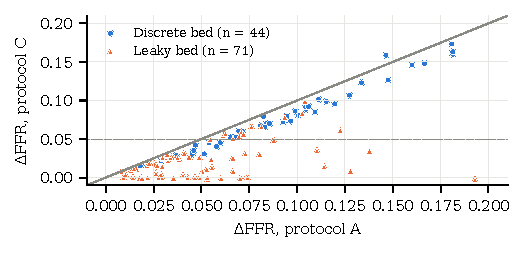
\includegraphics[width=0.55\textwidth]{figures/fig4_branch_loss.pdf}
\caption{Change in FFR caused by a missed side branch under fixed boundary conditions (Protocol A) and after tuning
to territory flows with one global scaling (Protocol C), paired by instance. The solid line is the identity and the
dashed line marks $\Delta$FFR $= 0.05$. Under per-territory tuning (Protocol D) the median shift was 0.000
(discrete) and 0.004 (leaky).}\label{fig:branch}
\end{figure}

\FloatBarrier
\section{Mixed-Effects Model of Flips}
\begin{table}[!ht]
\caption{Bayesian Mixed-Effects Logistic Model of Flips: Posterior Mean Log-Odds (95\% Interval)}\label{tab:glmm}
\centering\small
\begin{tabular}{@{}lcc@{}}
\toprule
Term & Discrete bed & Leaky bed\\
\midrule
\inputtab supplement_tables/tab_glmm.tex 
\bottomrule
\end{tabular}
\\[3pt]
\parbox{0.85\textwidth}{\footnotesize Reference levels: T1 (missed branch) and Protocol A. Baseline-band terms are
omitted from the table. Random intercepts for patient and lesion slot. Fitted by variational inference; intervals are
posterior mean $\pm 1.96$ posterior standard deviations from the variational approximation.}
\end{table}

At the reference levels the model agrees with the paired tests: under fixed boundary conditions a vessel break carries
higher odds of a flip than a missed branch and the caliber errors lower odds, and for the missed branch Protocols B and
C carry lower odds than Protocol A, in both beds. In the leaky bed the T2 $\times$ B and T2 $\times$ C interactions
offset the T2 main effect, so under re-derived or tuned boundary conditions the two topological errors have similar
odds, as in Table I of the main text.

\FloatBarrier
\section{Sensitivity Analyses}
\subsection{Perfusion-Check Threshold}
Table~\ref{tab:thr} repeats the proportion of models that pass the perfusion check while materially wrong at the
primary threshold of 10\% and at the 13\% and 16\% sensitivities, for the topological errors and for all error
types, and gives the number of models that pass at 10\% and the proportion of those that are materially wrong.
\begin{table}[!ht]
\caption{Proportion of Models That Pass the Perfusion Check and Are Materially Wrong, \% (Wilson 95\% Interval), by
Perfusion-Check Threshold}\label{tab:thr}
\centering\small
\begin{tabular}{@{}lllrcccrc@{}}
\toprule
 & & & & \multicolumn{3}{c}{Passes and wrong, \% of $n$} & \multicolumn{2}{c}{At 10\%}\\
\cmidrule(lr){5-7}\cmidrule(l){8-9}
Bed & Errors & Protocol & $n$ & 10\% & 13\% & 16\% & Pass & Wrong among passing, \%\\
\midrule
\inputtab supplement_tables/tab_thresholds.tex 
\bottomrule
\end{tabular}
\\[3pt]
\parbox{0.85\textwidth}{\footnotesize Materially wrong: $|\Delta\mathrm{FFR}| > 0.05$. The 13\% and 16\% thresholds were analyzed as sensitivities. $n$ counts models with a
defined perfusion residual: T2 under Protocols A and B in the leaky bed, $n = 100$; T2 under Protocol B in the
discrete bed, $n = 60$. Protocol D matches every territory flow, so its passes-and-wrong proportion equals its
materially wrong proportion.}
\end{table}

\FloatBarrier
\subsection{Hyperemic Demand}\label{sec:demand}
The demand constant $k$ was scaled by 0.7 and 1.3 and the full ablation was repeated with the same frozen cohort
(Table~\ref{tab:demand}). The ordering of topological against caliber errors under fixed boundary conditions, and of
Protocols B and C against Protocol A for the topological errors, was unchanged at both levels in both beds. The taper,
which flipped fewer decisions under Protocol C than under Protocol A at the primary demand, flipped one and two more
at 1.3 times the demand (7 against 6 of 97; 11 against 9 of 150). The magnitudes changed with demand, which moves the
clean FFR of every instance (leaky-bed median 0.869, 0.801 and 0.741 at 0.7, 1.0 and 1.3 times the demand) and
therefore the number of instances near the threshold, as well as the pressure loss across the lesion. The proportion
of tuned topological-error models that pass the perfusion check while materially wrong fell to 3\% in the leaky bed
at 0.7 times the demand, comparable with the simulated floor for correct anatomy (3.9\% at the primary demand); in
the discrete bed it remained between 12\% and 25\%.
\begin{table}[!h]
\caption{Sensitivity to Hyperemic Demand}\label{tab:demand}
\centering\small
\begin{tabular}{@{}llcccccc@{}}
\toprule
Bed & Demand scale & \multicolumn{2}{c}{Flip, \% (Protocol A)} & \multicolumn{2}{c}{Topological flip, \%} &
Passes and wrong, \% & Missed-branch $\Delta$FFR\\
\cmidrule(lr){3-4}\cmidrule(lr){5-6}
 & & Topological & Caliber & B & C & (C, topological) & median, A / C\\
\midrule
Discrete & 0.7 & 32 (25--40) & 6 (3--10) & 12 (8--18) & 18 (12--27) & 12 (7--19) & 0.070 / 0.057 \\
 & 1.0 & 33 (26--41) & 10 (7--15) & 14 (10--20) & 19 (13--28) & 19 (13--28) & 0.095 / 0.077 \\
 & 1.3 & 40 (32--48) & 5 (2--9) & 16 (11--22) & 19 (13--28) & 25 (18--34) & 0.106 / 0.091 \\
Leaky & 0.7 & 20 (16--26) & 6 (4--9) & 7 (4--10) & 9 (5--14) & 3 (1--7) & 0.032 / 0.010 \\
 & 1.0 & 32 (26--38) & 6 (4--9) & 5 (3--8) & 8 (5--13) & 8 (5--13) & 0.047 / 0.015 \\
 & 1.3 & 37 (32--43) & 4 (2--7) & 5 (3--9) & 8 (4--13) & 12 (8--18) & 0.057 / 0.021 \\
\bottomrule
\end{tabular}
\\[3pt]
\parbox{0.9\textwidth}{\footnotesize Demand scale 1.0 is the primary analysis ($k = 562$~s$^{-1}$). Percentages with Wilson 95\%
intervals in parentheses. Missed-branch $\Delta$FFR is over the instances in which Protocol C was defined.}
\end{table}


\FloatBarrier
\subsection{Demand Replication With Re-Selected Cohorts}\label{sec:replication}
Because hyperemic demand follows the segmented inlet radius, the modeled flow was below thermodilution values for
normal-sized arteries. The whole pipeline (stenosis sweep, stratified selection with the same rule and seed,
discrete-arm eligibility, Protocols A--D) was therefore repeated with $k$ doubled and tripled, so that the reselected
cohorts again span 0.80 at the higher flow. At three times the demand only 17 instances met the discrete-bed
eligibility criteria, mostly because the healthy-equivalent network lost more than 10\% of the aortic pressure, so the
discrete arm is reported at twice the demand only (Table~\ref{tab:repl}).
\begin{table}[!ht]
\caption{Demand Replication: Flip and Passes-and-Wrong Rates, \% (Wilson 95\% Interval)}\label{tab:repl}
\centering\footnotesize\setlength{\tabcolsep}{3pt}
\begin{tabular}{@{}lrrcccccccccc@{}}
\toprule
 & & & \multicolumn{2}{c}{Flip, A} & \multicolumn{2}{c}{Topological flip} & \multicolumn{3}{c}{Topological passes and wrong} & \multicolumn{3}{c}{Caliber passes and wrong}\\
\cmidrule(lr){4-5}\cmidrule(lr){6-7}\cmidrule(lr){8-10}\cmidrule(l){11-13}
Bed & $k$ scale & Inst. & Topol. & Caliber & C & D & B & C & D & B & C & D\\
\midrule
\inputtab supplement_tables/tab_replication.tex 
\bottomrule
\end{tabular}
\\[3pt]
\parbox{0.95\textwidth}{\footnotesize Scale 1 is the primary analysis ($k = 562$~s$^{-1}$, primary cohort). Scales 2 and 3 use
cohorts reselected at that demand. Passes and wrong: perfusion residual below 10\% and $|\Delta\mathrm{FFR}| > 0.05$;
denominators are models with a defined residual, as in Table I of the main text.}
\end{table}

\FloatBarrier
\subsection{Grey Zone}\label{sec:grey}
A change of classification at 0.80 between two values close to the threshold falls inside the diagnostic grey zone
of 0.75--0.85. Table~\ref{tab:grey} separates the flips that end beyond this zone, with the corrupted FFR outside
0.75--0.85 on the other side of 0.80 from the clean FFR. Of the clean models, 30\% (discrete) and 33\% (leaky) lay
inside the zone.
\begin{table}[!ht]
\caption{Flips and Flips Beyond the Grey Zone (0.75--0.85), \% of Models (Wilson 95\% Interval)}\label{tab:grey}
\centering\footnotesize
\begin{tabular}{@{}llrccrcc@{}}
\toprule
 & & \multicolumn{3}{c}{Topological errors} & \multicolumn{3}{c}{Caliber errors}\\
\cmidrule(lr){3-5}\cmidrule(l){6-8}
Bed & Protocol & $n$ & Flip & Beyond zone & $n$ & Flip & Beyond zone\\
\midrule
\inputtab supplement_tables/tab_greyzone.tex 
\bottomrule
\end{tabular}
\end{table}

\FloatBarrier
\section{Noise Floors}\label{sec:floor}
The repeat-measurement floor uses the published standard deviation of the test--retest difference in invasive FFR, 0.018. The simulated floor
uses the clean anatomy of every instance, with 20 draws per instance. Each draw perturbs cardiac output (relative
within-subject standard deviation 0.05), mean aortic pressure (0.056), blood viscosity through hematocrit (0.02), the
share of flow to each territory (0.10) and the measured territory flows (within-subject coefficient of variation
0.083), and the model is then tuned to the perturbed flows as in Protocol C. Heart rate is not represented in the
steady model. The territory-share and measurement terms lie at the low end of published ranges, so the simulated floor
may understate physiological variation. Table~\ref{tab:floor} gives the result. The repeat-measurement floor is
5.0--6.5\% across cells and the simulated floor 6.2\% and 7.2\%.
\begin{table}[!ht]
\caption{Simulated Floor: Correct Anatomy Tuned to Noisy Perfusion}\label{tab:floor}
\centering\small
\begin{tabular}{@{}lrrcccrc@{}}
\toprule
Bed & Instances & Draws solved & Flip, \% & Median $|\Delta$FFR$|$ & 95th pct. $|\Delta$FFR$|$ & Pass, \% &
Pass and wrong, \%\\
\midrule
\inputtab supplement_tables/tab_floor.tex 
\bottomrule
\end{tabular}
\end{table}

\FloatBarrier
\section{Three-Dimensional Case Study: Mesh Checks}\label{sec:cfd}
The mask-to-solution path was scripted with no manual repair, and the lesion-free, baseline and missed-branch solves
converged. Three acceptance rules were met with deviations. (i) The throat-size gate compared the ratio of the
as-built throat radius to the undeformed meshed radius with the intended radial scale (within 1\%), rather than the
absolute throat radius with the reduced-order target, because the two pipelines define the radius differently. (ii) A surface self-intersection flag arises from the segmentation mask, not from the mesher. (iii) The
strict mesh-quality check flags poorly shaped cells (face-tetrahedra decompositions) 1.43~mm from the throat center,
inside the planned 2~mm exclusion distance; the lesion-free mesh carries a similar count, and the standard quality
check passes. To test whether these cells affect the result, the baseline was re-meshed with a finer throat zone
(Table~\ref{tab:d7}). The acceptance criterion, a change smaller than the discretization uncertainty of
$5.5\times10^{-4}$, was not met: the finer zone raised the measurement-point FFR by 0.0019 and 0.0021, while a
regenerated mesh at the production resolution reproduced the original value. The second variant missed the strict
residual limit at the iteration budget (final velocity residual $1.08\times10^{-5}$ against $10^{-5}$) with its inlet
pressure steady to $4\times10^{-4}$~Pa over the last 500 iterations; its value is reported as returned. This is a resolution sensitivity of
about 0.2\% of the FFR, against an error effect of 0.074 in the same case.

All 3D-to-0D comparisons use a reduced-order counterpart rebuilt on the meshed radius, which is wider than the
reduced-order radius (main text, Section III-D).
\begin{table}[!ht]
\caption{Throat-Zone Resolution Test, Baseline Lumen. The 8.31~M-cell mesh did not meet the strict residual limit at
3\,000 iterations (see text).}\label{tab:d7}
\centering\small
\begin{tabular}{@{}lrrrrr@{}}
\toprule
Mesh & Cells (M) & FFR & $\Delta$FFR & Outlet flow change, \% & Flagged cell to throat, mm\\
\midrule
\inputtab supplement_tables/tab_d7.tex 
\bottomrule
\end{tabular}
\end{table}

\end{document}
